% !TEX root = main.tex

\section{简介}

\subsection{实验目的}

\begin{itemize}[noitemsep]
    \item 理解高速缓存(Cache)的工作原理, 掌握常见的映射方式和替换策略.
    \item 学会针对Cache对程序代码进行优化.
\end{itemize}

\subsection{实验要求}

\begin{itemize}
  \item Part A: \\编写一个Cache模拟器 \verb|csim| , 支持任意参数的组相连映射(Set associative), 采用最近最少使用(Least recently used)替换策略, 功能应当与给定的参考程序 \verb|csim-ref| 一致.
  \item Part B: \\优化一个矩阵转置函数, 尽可能减少Cache misses, 提高Cache命中率. 考虑 $32 \times 32$, $ 64 \times 64$ 和 $ 61 \times 67$ 三种情形. 要求遵守给定的编程规则.
\end{itemize}

\subsection{实验环境}

本实验Part A在以下环境完成:
\begin{center}
    \small
    \begin{tabular}{ll}
      \toprule
      Machine & MacBook Pro 13" \\
      SoC & Apple M1, 基于ARM, 含8核CPU、8核GPU及16GB RAM \\
      OS & macOS Monterey 12.4 \\
      IDE & Visual Studio Code 1.68.1 \\
      Docker & Docker 20.10.13 \\
      Image & Ubuntu 22.04, amd64 \\
      Packages & GCC 11.2.0, Make 4.3, Python 2.7.18, Valgrind 3.18.1\\
      \bottomrule
    \end{tabular}
\end{center}

容器配置参见附录 \ref{codelist} \nameref{dockerfile}.

\clearpage
\section{实验成果}
由于时间不足与设备问题\footnote{在ARM机器上使用QMEU仿真amd64架构, 无法正常运行 \texttt{valgrind}, \texttt{gdb} 等跟踪调试工具.}, Part B 尚未完成.
Part A的测试结果如\figref{result} 所示.

\begin{figure}[H]
    \centering
    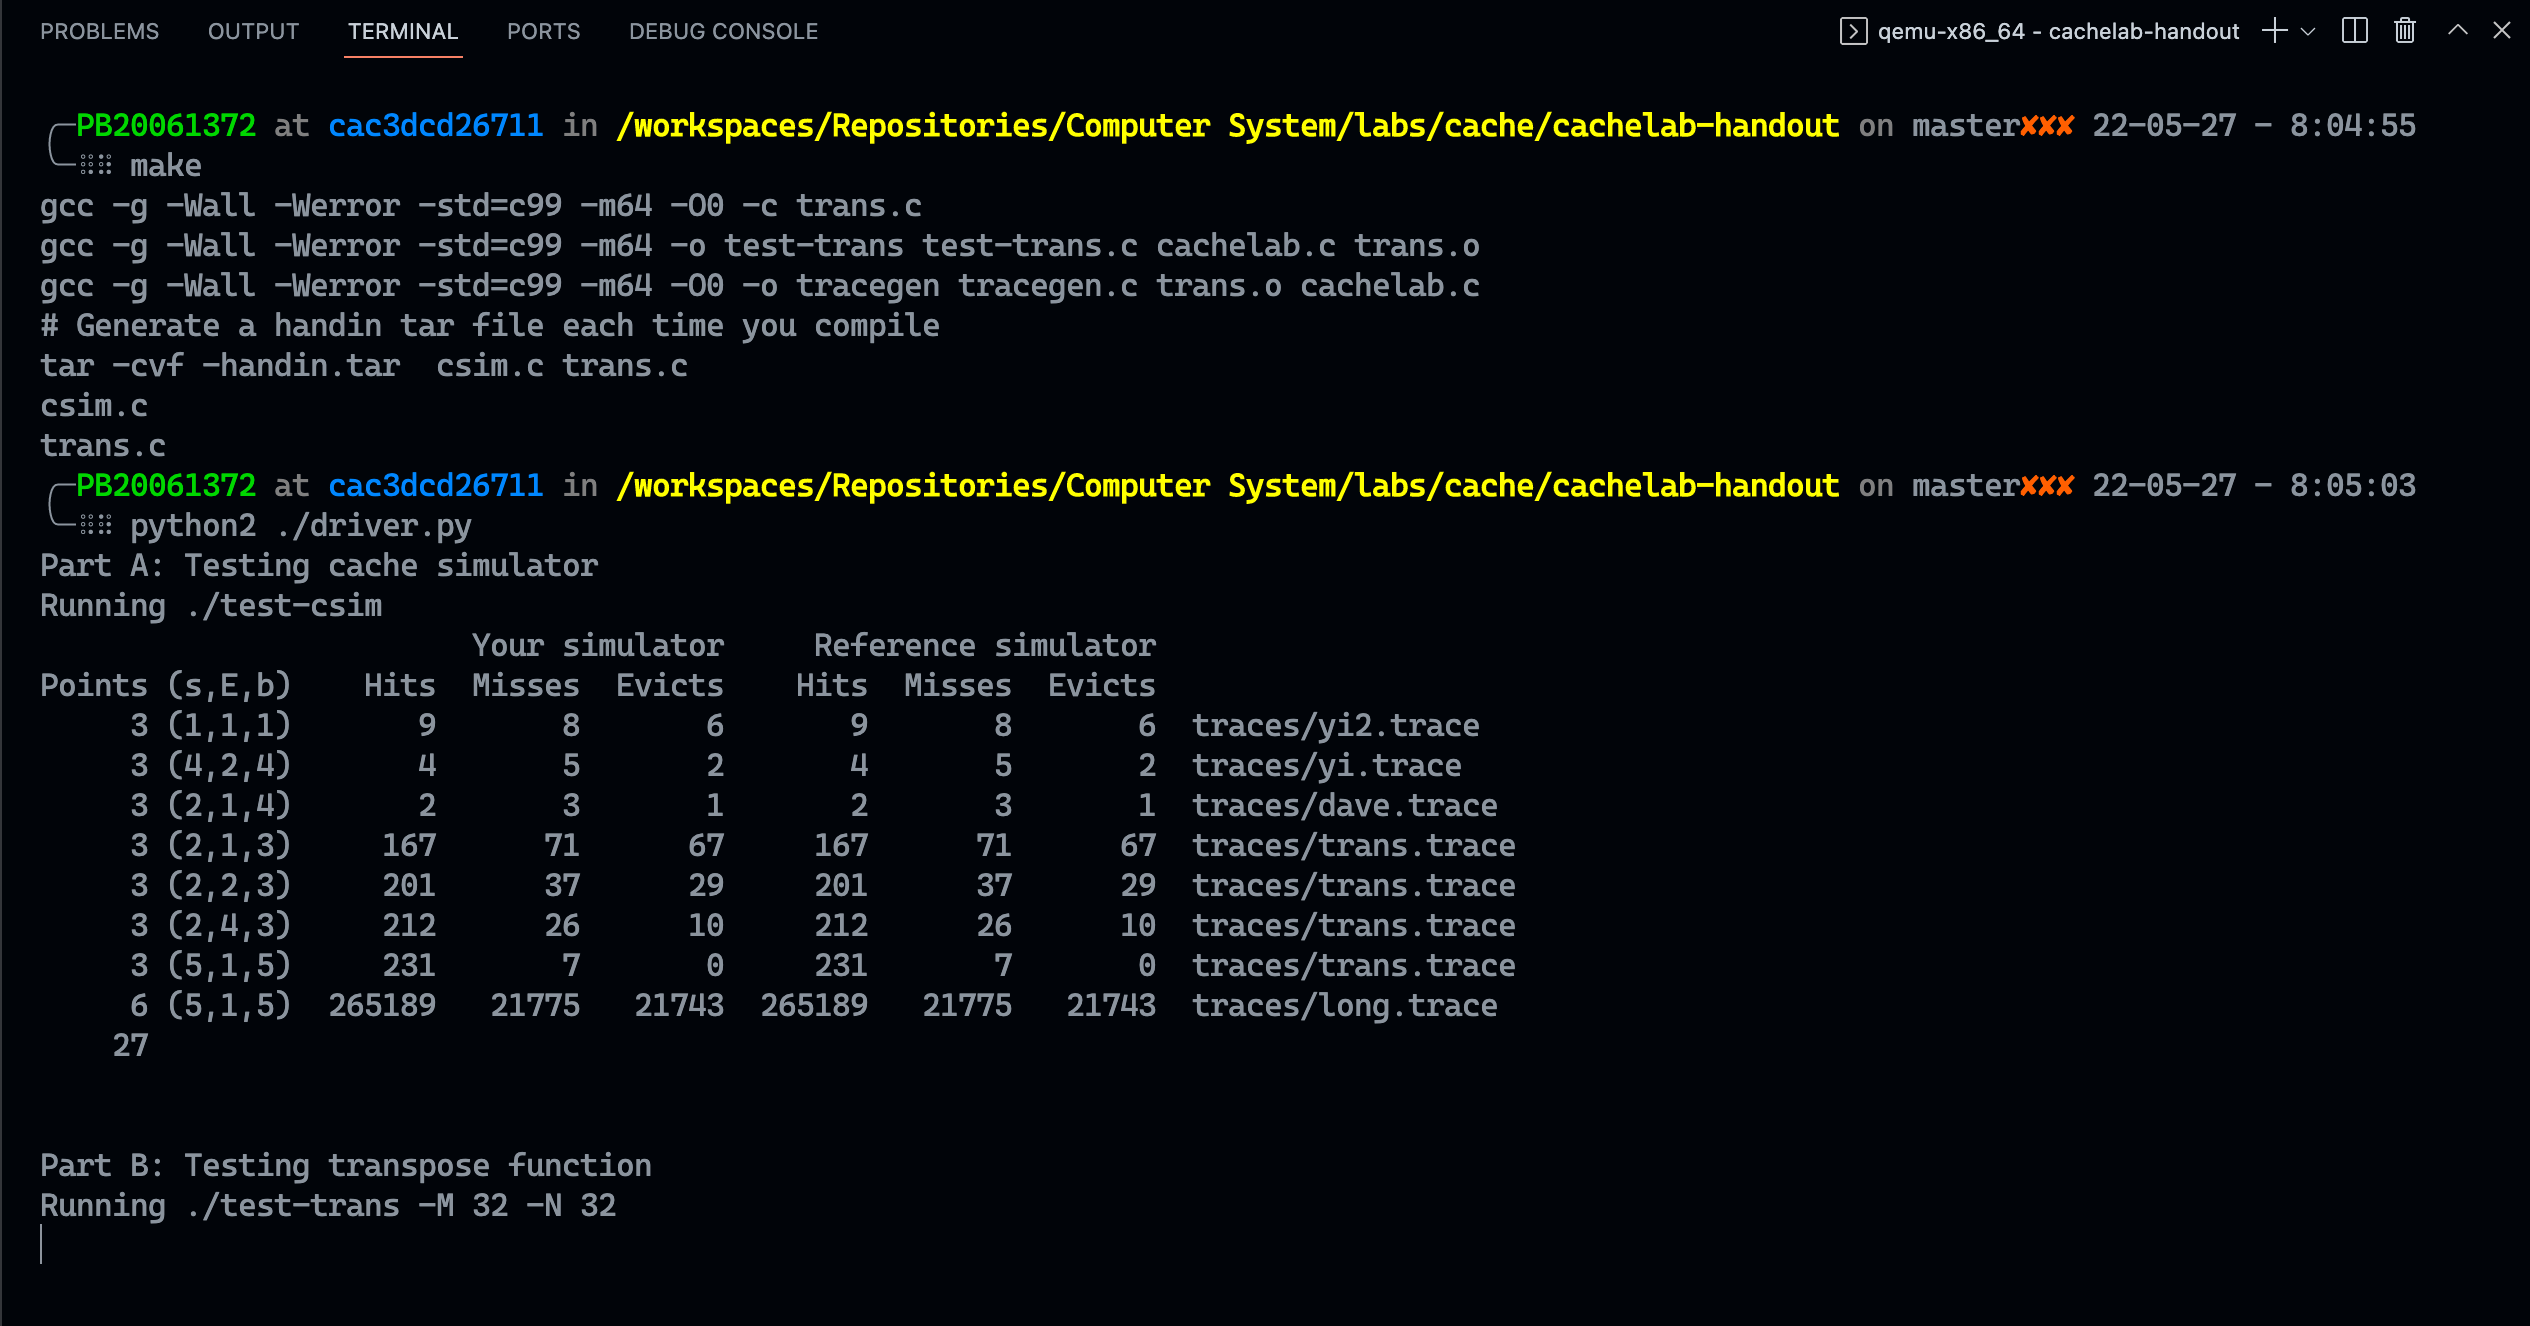
\includegraphics[width=0.8\textwidth]{result.png}
    \caption{在终端中运行 \texttt{driver.py}, 验证Part A的正确性}\label{result}
\end{figure}

完整源文件, 参见附录 \ref{codelist} \nameref{csim-c}.

\section{实验过程}

\subsection{Part A: 工作原理}\label{principle}

采用组相连映射方案, Cache结构如\figref{cache-org} 所示. 

\begin{figure}[H]
  \centering
  \begin{tikzpicture}[
    node distance = 0pt,
    every node/.style = {
        inner sep = 0pt,
        outer sep = 0pt
    },
    every matrix/.style = {
        inner sep = 0pt,
        outer sep = 0pt
    },
  ]{
    \matrix (cache) [
        anchor = north,
        row sep = 5pt,
        column sep = 5pt,
        nodes = {rect, minimum width=50pt},
        left delimiter = \{,
        above delimiter = \{
    ]{
        \node {}; & \node {}; & \node [draw=none]{......}; & \node {}; \\
        \node {}; & \node {}; & \node [draw=none]{......}; & \node {}; \\
        \node {}; & \node {}; & \node [draw=none]{......}; & \node {}; \\
        \node [draw=none]{......}; & \node [draw=none]{......}; & \node [draw=none]{......}; & \node [draw=none]{......}; \\
        \node {}; & \node (cache line){}; & \node [draw=none]{......}; & \node (last){}; \\
    };
    \node at (-28pt, -150pt)(Cache line)[
        draw, thick, 
        minimum height = 20pt,
        minimum width = 170pt
        ]{};
    \matrix [
        left = -60pt of Cache line,
        column sep = 5pt,
        nodes = {rect, minimum height=15pt}
    ]{
        \node (valid bit)[minimum width=15pt]{v}; & \node [minimum width=30pt]{tag}; \\
    };
    \matrix (cache block)[
        right = -100pt of Cache line,
        column sep = -0.8pt,
        nodes = {rect, minimum height=15pt, minimum width=15pt},
        below delimiter = \}
    ]{
        \node {}; & \node {}; & \node {}; & \node [minimum width=30pt]{......}; & \node {}; \\
    };
    \matrix (address)[
        right = 40pt of cache,
        column sep = -0.8pt,
        nodes = {rect},
    ]{
        \node (tag)[minimum width=30pt, label=above:$t$ bits]{tag}; & \node (set index)[minimum width=60pt, label=above:$s$ bits]{set index}; & \node (block offset)[minimum width=70pt, label=above:$b$ bits]{block offset}; \\
    };
    \node [left=16pt of cache]{$S=2^s$ sets};
    \node [above=16pt of cache]{$E=2^e$ lines per set};
    \node [below=12pt of cache block]{$B=2^b$ bytes per block};
    \node [below=14pt of valid bit]{valid bit};
    \draw (-53pt,-123pt) to (-103pt,-140pt);
    \draw (-3pt,-123pt) to (47pt,-140pt);
    \draw[trace] (-96pt,-160pt) to (-96pt,-170pt);
    \draw[trace] (set index) |- (last);
    \draw[trace] (block offset) |- (cache block);
  }
  \end{tikzpicture}
  \caption{Cache的组成结构}\label{cache-org}
\end{figure}

Cache空间被分为$2^s$个组(set),每个组含有$E$个行(line), 称作$E$路组相连. cache line由一个有效位(valid bit),标签(tag)以及$2^b$个字的数据块(block)组成. 

在Cache的硬件实现中, CPU每次访问内存, 内存地址被划分为tag, set index, block offset三部分. 在set index对应的组中, 逐个比较有效cache line的tag与地址中的tag, 若匹配则Cache命中, 根据block offset访问数据; 若未命中, 按照某种策略替换cache line内容.

通常采用LRU替换策略. 为每个cache line增设一个计数值, 当一个cache line被访问时, 其计数值归零, 其余的有效cache line计数值加一. 每次Cache未命中而Cache已满时, 优先替换计数值最大的cache line.

\subsection{Part A: 程序流程}

根据Cache工作原理以及实验材料的提示, 设计得程序流程大致如\figref{flowchart} 所示.

\begin{figure}[H]
  \centering
  \begin{tikzpicture}{
    \node (start)[startstop]{Start \texttt{csim.c}};
    \node (input)[io=3cm, left=3cm of start]{Input $s$, $E$, $b$, etc. as args};
    \node (parse)[process,below=of input]{Parse args};
    \node (init)[process,below=of parse]{Allocate memory for cache};
    \node (read)[process,below=of init]{Read an operation from trace file};
    \node (access)[process,right=of read]{Parse the operation and access the cache};
    \node (eof)[decision,below=of access]{End of trace file?};
    \node (deinit)[process,below=of eof]{Deallocate memory for cache};
    \node (output)[io=3cm,below=of deinit]{Output number of hits and misses};
    \node (stop)[startstop, left=3cm of output]{End \texttt{csim.c}};
    \draw[trace] (start) -- (input);
    \draw[trace] (input) -- (parse);
    \draw[trace] (parse) -- (init);
    \draw[trace] (init) -- (read);
    \draw[trace] (read) -- (access);
    \draw[trace] (access) -- (eof);
    \draw[trace] (eof) -- (deinit) node[pos=0.5,fill=white,inner sep=0]{Yes};
    \draw[trace] (eof) -| (read) node[pos=0.25,fill=white,inner sep=0]{No};
    \draw[trace] (deinit) -- (output);
    \draw[trace] (output) -- (stop);
    }
  \end{tikzpicture}
  \caption{Cache模拟程序的流程图}\label{flowchart}
\end{figure}

主函数的代码如下:
\begin{code}{c}
int main(int argc, char *argv[]) {
  parseArgs(argc, argv);
  initCache();
  FILE *trace_fp = fopen(trace_file, "r");

  char line[32];
  while (fgets(line, 32, trace_fp)) {
    /* Ignore instruction cache accesses */
    if (line[0] == 'I')
      continue;

    /* Parse operation */
    char op;
    unsigned int addr;
    int size;
    sscanf(line, " %c %x,%d", &op, &addr, &size);

    accessCache(op, addr, size);
  }

  fclose(trace_fp);
  deinitCache();
  printSummary(num_hits, num_misses, num_evictions);
  return 0;
}
\end{code}

\subsection{Part A: 处理命令行参数}

首先考虑如何处理命令行参数. 根据参考程序 \verb|csim-ref| 的功能, 并遵循 \verb|test_trans.c| 的编程风格, 不妨用如下 \verb|usage| 函数打印帮助信息:

\begin{code}{c}
 *argv[]) {
  printf("Usage: %s [-hv] -s <num> -E <num> -b <num> -t <file>", argv[0]);
  printf("Options:\n");
  printf("  -h         Print this help message.\n");
  printf("  -v         Optional verbose flag.");
  printf("  -s <num>   Number of set index bits.\n");
  printf("  -E <num>   Number of lines per set.\n");
  printf("  -b <num>   Number of block offset bits.\n");
  printf("  -t <file>  Trace file.\n");
  printf("\n");
  printf("Examples:\n");
  printf("  linux>  %s -s 4 -E 1 -b 4 -t traces/yi.trace\n", argv[0]);
  printf("  linux>  %s -v -s 8 -E 2 -b 4 -t traces/yi.trace\n", argv[0]);
}
\end{code}

程序支持 \verb|-h|, \verb|-v| 两个可选项, 分别用于显示帮助信息和设置是否打印详细信息. \verb|-s|, \verb|-E|, \verb|-b| 为必需参数, 已在\nameref{principle}中解释. \verb|-t| 也为必需参数, 用于指定跟踪文件.

设置如下全局变量用于存储上述参数:
\begin{code}{c}
/* Globals set on the command line */
static int s = 0; // Number of set index bits
static int E = 0; // Number of lines per set
static int b = 0; // Number of block offset bits
static int verbose_mode = 0;
static char *trace_file = NULL;
\end{code}

根据提示, 可用 \verb|getopt| 库函数解析命令行参数. 遵循 \verb|test_trans.c| 的编程风格, 编写如下 \verb|parseArgs| 函数:
\begin{code}{c}
void parseArgs(int argc, char *argv[]) {
  char c;

  while ((c = getopt(argc, argv, "hvs:E:b:t:")) != -1) {
    switch (c) {
    case 's':
      s = atoi(optarg);
      break;
    case 'E':
      E = atoi(optarg);
      break;
    case 'b':
      b = atoi(optarg);
      break;
    case 't':
      trace_file = optarg;
      break;
    case 'v':
      verbose_mode = 1;
      break;
    case 'h':
      usage(argv);
      exit(0);
    default:
      usage(argv);
      exit(1);
    }
  }
}
\end{code}

\subsection{Part A: 分配内存空间}

视命令行参数不同, Cache大小也不同, 需要动态分配内存. 首先, 给出用于存储Cache的结构体:
\begin{code}{c}
/* Struct for cache lines */
typedef struct cache_line {
  int count; // Number of times this line has been accessed
  int valid;
  unsigned int tag;
} cache_line_t, *cache_set_t, **cache_t;
static cache_t cache;
\end{code}

本实验仅要求模拟Cache的命中与否, 无需对数据进行操作, 因此 \verb|cache_line| 结构体不含数据块. 此外, 为了实现LRU替换策略, 增设了一个计数值 \verb|count|. 

每个set视为cache line数组, Cache视为set数组. 不难编写 \verb|initCache| 和 \verb|deinitCache| 函数, 分别用于创建与销毁Cache.

\begin{code}{c}
void initCache() {
  int S = 1 << s; // Number of sets
  cache = malloc(sizeof(cache_set_t) * S);
  for (int i = 0; i < S; i++)
    cache[i] = calloc(E, sizeof(cache_line_t));
}

void deinitCache() {
  int S = 1 << s; // Number of sets
  for (int i = 0; i < S; i++)
    free(cache[i]);
  free(cache);
}
\end{code}

\subsection{Part A: 模拟Cache访问}

Cache的访问和更新, 由以下 \verb|accessCache| 函数实现:
\begin{code}{c}
void accessCache(char op, unsigned int addr, int size) {

  /* Calculate tag in address */
  unsigned int tag = addr >> (s + b);
  /* Get cache set by index */
  cache_set_t set = cache[addr >> b & ((1 << s) - 1)];

  /* 'M' operation always results in an extra hit */
  if (op == 'M')
    num_hits++;

  if (verbose_mode)
    printf("%c %x,%d ", op, addr, size);

  /* Check if there is a hit */
  int empty = -1, lru = 0;
  for (int i = 0; i < E; i++) {
    if (!set[i].valid)
      empty = i; // Search for an empty line
    else if (set[i].tag == tag) {
      if (verbose_mode)
        printf(op == 'M' ? "hit hit\n" : "hit\n");
      num_hits++;
      set[i].count = 0; // Update time count using LRU policy
      return;
    } else if (++set[i].count >= set[lru].count)
      lru = i; // Search for the LRU line
  }

  /* If there is no empty line, evict the LRU line */
  cache_line_t *line;
  if (empty >= 0) {
    if (verbose_mode)
      printf(op == 'M' ? "miss hit\n" : "miss\n");
    line = &set[empty];
  } else {
    if (verbose_mode)
      printf(op == 'M' ? "miss eviction hit\n" : "miss eviction\n");
    line = &set[lru];
    num_evictions++;
  }
  line->valid = 1;
  line->tag = tag;
  line->count = 0;
  num_misses++;
}
\end{code}

根据\figref{cache-org}, 不难得到由地址获取tag与set index的位操作表达式:
\begin{center}
  \verb|tag = addr >> (s + b)| \\
  \verb|set_index = addr >> b & ((1 << s) - 1)|
\end{center}

随后循环匹配tag, 与此同时查找空行与最近最少使用的行. 使用三个全局变量 (\verb|num_hits| 等) 记录统计数据, 适时更新. 对于跟踪文件中的数据调整操作(以\verb|‘M’|开头), 本质为先读后写, 应当额外考虑.

至此, 实现了Cache模拟器, 测试结果参见\figref{result}.

\subsection{Part B: 第一次尝试}
To be continued...

\subsection[Part B: 针对32 x 32情形优化]{Part B: 针对$32 \times 32$情形优化}
To be continued...

\subsection[Part B: 针对64 x 64情形优化]{Part B: 针对$64 \times 64$情形优化}
To be continued...

\subsection[Part B: 针对61 x 67情形优化]{Part B: 针对$61 \times 67$情形优化}
To be continued...

\section{总结}

完成Cache Lab, 主要有以下收获:
\begin{itemize}
    \item 深入理解了内存访问的时空局部性, Cache的原理和意义;
    \item 掌握了Cache的组成结构, 与主存的映射方式;
    \item 掌握了组相连映射的思想, 能够定量分析映射过程;
    \item 掌握了LRU替换策略的思想, 能够自行通过软件实现;
    \item 体会了Cache对程序性能的影响, 明白了代码优化的重要性;
    \item 学会了矩阵转置算法中, 针对Cache进行优化的几种途径;
    \item 学会了使用 \verb|getopt| 库函数解析命令行参数;
\end{itemize}
本实验的所有材料已上传至GitHub:

\url{https://github.com/HasiNed/Computer-System}

\setupappendix

\clearpage
\section{代码清单}\label{codelist}

\subsection{\texttt{csim.c}}\label{csim-c}
\includecode{c}{../cachelab-handout/csim.c}

\subsection{\texttt{Dockerfile}}\label{dockerfile}
\includecode{dockerfile}{Dockerfile}